\documentclass[aspectratio=169]{beamer}

\usetheme{Madrid}
\usecolortheme{seahorse}
\usepackage{listings}
\usepackage{tikz}
\usetikzlibrary{arrows.meta, shapes.geometric, positioning, fit, backgrounds}
\usepackage{booktabs}
\usepackage{xcolor}
\usepackage{graphicx}

% color palette
\definecolor{zblue}{RGB}{31, 78, 121}
\definecolor{zaccent}{RGB}{0, 112, 192}
\definecolor{zwarn}{RGB}{192, 80, 77}
\definecolor{zok}{RGB}{70, 130, 80}
\definecolor{zgray}{RGB}{89, 89, 89}
\definecolor{codebg}{RGB}{245, 246, 250}
\definecolor{dqone}{RGB}{0, 90, 156}
\definecolor{dqtwo}{RGB}{130, 60, 10}

\setbeamercolor{frametitle}{bg=zblue, fg=white}
\setbeamercolor{title}{bg=zblue, fg=white}
\setbeamercolor{structure}{fg=zaccent}
\setbeamercolor{block title}{bg=zblue!80, fg=white}
\setbeamercolor{block body}{bg=zblue!8}
\setbeamercolor{alerted text}{fg=zwarn}

\lstdefinestyle{json}{
  basicstyle=\ttfamily\scriptsize,
  backgroundcolor=\color{codebg},
  frame=single, framerule=0.4pt, rulecolor=\color{zaccent!40},
  xleftmargin=4pt, xrightmargin=4pt,
  breaklines=true, showstringspaces=false
}

% Simple inline design-question labels; avoid box environments to prevent LR-mode errors
\newcommand{\dqone}[1]{%
  \par\vspace{0.35em}%
  \noindent{\small\color{dqone}\textbf{Q\textsubscript{1}:} \textit{#1}}%
  \par\vspace{0.1em}%
}
\newcommand{\dqtwo}[1]{%
  \par\vspace{0.35em}%
  \noindent{\small\color{dqtwo}\textbf{Q\textsubscript{2}:} \textit{#1}}%
  \par\vspace{0.1em}%
}

\title{ZandrEA: Design Ideas}
\subtitle{Self-describing tools, flexible write path, S223 integration}
\author{}
\date{\today}

% ─────────────────────────────────────────────────────────────────────────────
\begin{document}

\begin{frame}
  \titlepage
\end{frame}

\begin{frame}{Roadmap}
  \tableofcontents
\end{frame}

% ─────────────────────────────────────────────────────────────────────────────
\section{Two Insert Paths}

\begin{frame}{Two independent insert paths}

\begin{center}
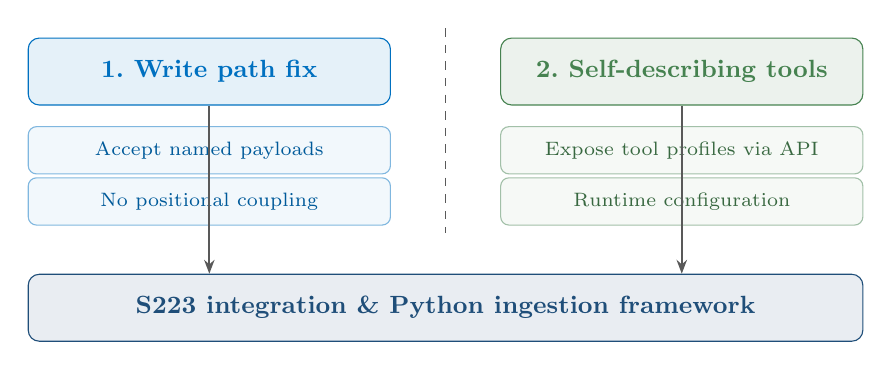
\begin{tikzpicture}[
  boxa/.style={rectangle, rounded corners=4pt, draw=zaccent, fill=zaccent!10,
               minimum width=4.6cm, minimum height=0.85cm,
               align=center, font=\small\bfseries, text=zaccent},
  boxb/.style={rectangle, rounded corners=4pt, draw=zok, fill=zok!10,
               minimum width=4.6cm, minimum height=0.85cm,
               align=center, font=\small\bfseries, text=zok},
  boxc/.style={rectangle, rounded corners=4pt, draw=zblue, fill=zblue!10,
               minimum width=10.6cm, minimum height=0.85cm,
               align=center, font=\small\bfseries, text=zblue},
  suba/.style={rectangle, rounded corners=3pt, draw=zaccent!50, fill=zaccent!5,
               minimum width=4.6cm, minimum height=0.6cm,
               align=center, font=\scriptsize, text=zaccent!80!black},
  subb/.style={rectangle, rounded corners=3pt, draw=zok!50, fill=zok!5,
               minimum width=4.6cm, minimum height=0.6cm,
               align=center, font=\scriptsize, text=zok!80!black},
  arr/.style={-{Stealth[length=5pt]}, thick, zgray}
]

\node[boxa] (ws1)  at (0,0)     {1.\ Write path fix};
\node[suba] (ws1a) at (0,-1.0)  {Accept named payloads};
\node[suba] (ws1b) at (0,-1.65) {No positional coupling};

\node[boxb] (ws2)  at (6.0,0)   {2.\ Self-describing tools};
\node[subb] (ws2a) at (6.0,-1.0)  {Expose tool profiles via API};
\node[subb] (ws2b) at (6.0,-1.65) {Runtime configuration};

\draw[zgray, dashed] (3.0,0.55) -- (3.0,-2.05);

\node[boxc] (s223) at (3.0,-3.0)
  {S223 integration \& Python ingestion framework};

\draw[arr] (ws1.south) -- (ws1.south |- s223.north);
\draw[arr] (ws2.south) -- (ws2.south |- s223.north);

\end{tikzpicture}
\end{center}

\vspace{0.2em}
\small Insert path 1 is a small change to \texttt{handler.cpp} and \texttt{CController}.
Insert path 2 is larger but modular.

\end{frame}

% ─────────────────────────────────────────────────────────────────────────────
\section{Write Path Fix}

\begin{frame}[fragile]{Insert path 1: Named payload}

\begin{columns}[T]
\column{0.48\textwidth}

\textbf{Today} --- positional array:
\begin{lstlisting}[style=json]
{
  "subject": 618,
  "values": [13.26, 24.21, 26.70, ...]
}
\end{lstlisting}

\vspace{0.5em}
\textbf{Proposed} --- named payload:
\begin{lstlisting}[style=json]
{
  "subject": 618,
  "values": {
    "Temperature_air_supply": 13.26,
    "Temperature_air_zone":   26.70,
    "Position_valve_hw":       0.0
  }
}
\end{lstlisting}

\column{0.48\textwidth}
\vspace{0.4em}
\texttt{handler.cpp} iterates over the registered point names for that subject, looks each up in the payload dict, and assembles \texttt{dlist} in the correct order. Everything downstream of \texttt{SetCoincidentInputsForSubject} is unchanged.

\vspace{0.5em}
Could keep the positional form working via an \texttt{app\_id} field specifying the tool type, so the server knows which ordering to assume.

\dqone{Support named payloads, positional+\texttt{app\_id}, or both?}

\end{columns}
\end{frame}

% ─────────────────────────────────────────────────────────────────────────────
\section{Tool Profiles}

\begin{frame}{Insert path 2: Tool profiles}

A \textbf{tool profile} describes what a tool type is and what data it requires.
Currently this lives only in the C++ constructor body.

\vspace{0.4em}
\begin{center}
\small
\begin{tabular}{lll}
\toprule
\textbf{Tool type} & \textbf{Class} & \textbf{Required points} \\
\midrule
VAV     & \texttt{CTool\_vav\_ibal}  & 11 points (10 analog, 1 binary) \\
AHU     & \texttt{CTool\_ahu\_ibal}  & 11 points (10 analog, 1 binary) \\
Chiller & \texttt{CTool\_chlr\_ibal} & 18 points (16 analog, 2 binary) \\
TES     & \texttt{CTool\_tes\_ibal}  & 6 points (6 analog) \\
\bottomrule
\end{tabular}
\end{center}

\vspace{0.4em}
Proposed API calls:
\begin{itemize}
  \item \texttt{GET /tools} --- list available tool types and their required points
  \item \texttt{GET /tools/\{type\}/points} --- full point list for a given tool type
\end{itemize}

\dqone{What is the identifier for a tool type in the API? Class name string? A short slug (\texttt{vav}, \texttt{ahu})?}
\dqtwo{Do profiles need to be compiled in, or can they be provided at runtime via config file or API?}

\end{frame}

\begin{frame}{Per-type vs per-instance profiles}

\begin{itemize}
  \item \textbf{Per-type}: all VAVs share one profile; a client fetches the VAV profile and knows what any instance needs
    \begin{itemize}
      \item Sufficient when all instances of a tool type have the same sensor configuration (what we have today)
    \end{itemize}
  \item \textbf{Per-instance}: each subject has its own point list; VAV-1 might have a CO\textsubscript{2} sensor, VAV-2 might not
    \begin{itemize}
      \item More expressive; requires the server to store a profile per subject key rather than per type
      \item Becomes relevant if once tool configuration is runtime-driven
      \item Example: a S223 model may describe two VAVs with different sensor sets
    \end{itemize}
\end{itemize}

\end{frame}

% ─────────────────────────────────────────────────────────────────────────────
\section{EPointName as API Contract}

\begin{frame}{\texttt{EPointName} strings as the API contract}

Use \texttt{EPointName} enum strings as identifiers for the required points in the tool profiles. These are already used in the C++ code as the internal contract between the controller and tools, so exposing them via an API endpoint is a small step that would allow clients to discover what points are needed without needing the header file.

\begin{center}
\footnotesize
\begin{tabular}{p{5.5cm} p{6.5cm}}
\toprule
\textbf{EPointName string} & \textbf{Physical meaning} \\
\midrule
\texttt{Temperature\_air\_supply}   & Supply air temperature \\
\texttt{Position\_damper\_vav}      & VAV damper position \\
\texttt{FlowRateVolume\_air\_vav}   & Airflow through VAV \\
\texttt{Binary\_zoneOccupied}       & Zone occupancy signal \\
\texttt{Temperature\_air\_zone\_setpt\_htg} & Heating setpoint \\
\bottomrule
\end{tabular}
\end{center}

\begin{itemize}\setlength{\itemsep}{0pt}\setlength{\parskip}{0pt}
  \item Strings are already the internal contract in the C++ code; exposing them in the API costs nothing
  \item Longer term, S223 concepts could map onto these strings --- e.g.\ \texttt{FlowRateVolume\_air\_vav} $\leftrightarrow$ a SHACL shape over an S223 model
\end{itemize}

\end{frame}

% ─────────────────────────────────────────────────────────────────────────────
\section{S223 Integration}

\begin{frame}{S223 integration: where does it live?}

\small From an S223 model, ZandrEA could automatically derive:
\begin{itemize}\setlength{\itemsep}{1pt}
  \item \textbf{Topology} --- which VAV serves which zone, which AHU serves which VAVs, etc.. Replaces the hardcoded topology in \texttt{CApplication}.
  \item \textbf{Data streams} --- what sensors are present per equipment and what they measure. Replaces manually assembled CSVs.
\end{itemize}

\vspace{0.1em}
\small\textbf{Where would the S223 model live?}
\begin{itemize}\setlength{\itemsep}{1pt}
  \item \textbf{Compiled into the server} --- same as today. Simple, but changing the model means recompiling.
  \item \textbf{Loaded at runtime by the server} --- server reads an S223 file at startup. Model is decoupled from the binary.
  \item \textbf{Uploaded by the Python client} --- client reads S223, translates it into ZandrEA API calls. Server stays simple; all S223 logic lives in the client.
\end{itemize}

\small ZandrEA doesn't need to become S223-exclusive. The \texttt{EPointName} strings remain the interface; S223 is one path to populate them automatically.

\end{frame}

% ─────────────────────────────────────────────────────────────────────────────
\section{Python Ingestion Framework}

\begin{frame}{Python ingestion}

\begin{columns}[T]
\column{0.50\textwidth}
\small
\begin{itemize}\setlength{\itemsep}{1pt}
  \item Fetch tool profiles from ZandrEA (\texttt{GET /tools})
  \item Map data sources (CSV columns, S223 streams) to required point names
  \item Validate mapping against the tool profile before uploading
  \item Post named-payload time steps to \texttt{/ctrl/sampletimestep}
  \item Suggest column mappings via heuristics or embeddings
\end{itemize}

\column{0.48\textwidth}

\begin{center}
\resizebox{\linewidth}{!}{%
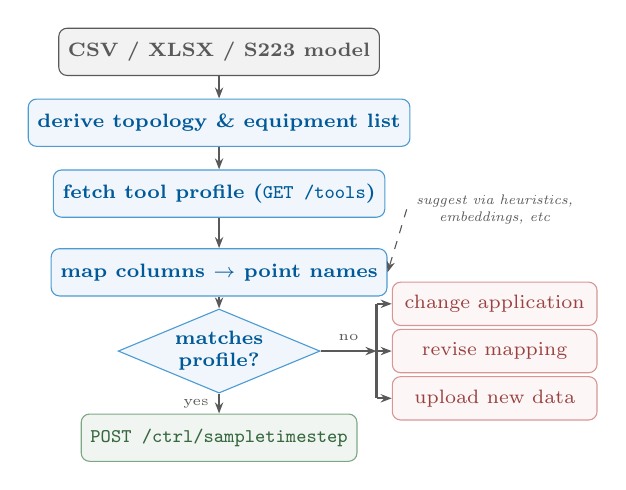
\begin{tikzpicture}[
  stepbox/.style={rectangle, rounded corners=3pt, draw=zaccent!70, fill=zaccent!6,
                  minimum width=3.4cm, minimum height=0.6cm,
                  align=center, font=\scriptsize\bfseries, text=zaccent!80!black},
  srcbox/.style={rectangle, rounded corners=3pt, draw=zgray, fill=zgray!8,
                 minimum width=3.4cm, minimum height=0.6cm,
                 align=center, font=\scriptsize\bfseries, text=zgray},
  decbox/.style={diamond, aspect=2.4, draw=zaccent!70, fill=zaccent!6,
                 align=center, font=\scriptsize\bfseries, text=zaccent!80!black,
                 inner sep=1pt},
  endbox/.style={rectangle, rounded corners=3pt, draw=zok!70, fill=zok!8,
                 minimum width=3.4cm, minimum height=0.6cm,
                 align=center, font=\scriptsize\bfseries, text=zok!80!black},
  failbox/.style={rectangle, rounded corners=3pt, draw=zwarn!60, fill=zwarn!5,
                  minimum width=2.6cm, minimum height=0.55cm,
                  align=center, font=\scriptsize, text=zwarn!80!black},
  hintbox/.style={font=\tiny\itshape, text=zgray, align=center},
  arr/.style={-{Stealth[length=4pt]}, thick, zgray},
  darr/.style={-{Stealth[length=4pt]}, zgray, dashed}
]

% Main vertical flow
\node[srcbox]  (src)  at (0,0)    {CSV / XLSX / S223 model};
\node[stepbox] (topo) at (0,-0.9) {derive topology \& equipment list};
\node[stepbox] (prof) at (0,-1.8) {fetch tool profile (\texttt{GET /tools})};
\node[stepbox] (map)  at (0,-2.8) {map columns $\to$ point names};
\node[decbox]  (dec)  at (0,-3.8) {matches\\profile?};
\node[endbox]  (post) at (0,-4.9) {\texttt{POST /ctrl/sampletimestep}};

% Hint beside map step (further right)
\node[hintbox] (hint) at (3.5,-2.0) {suggest via heuristics,\\embeddings, etc};

% Failure options to the right of decision
\node[failbox] (f1) at (3.5,-3.2) {change application};
\node[failbox] (f2) at (3.5,-3.8) {revise mapping};
\node[failbox] (f3) at (3.5,-4.4) {upload new data};

% Junction point for the no-branch
\coordinate (junc) at (2.0,-3.8);

% Main flow arrows
\draw[arr] (src)  -- (topo);
\draw[arr] (topo) -- (prof);
\draw[arr] (prof) -- (map);
\draw[arr] (map)  -- (dec);
\draw[arr] (dec)  -- node[left, font=\tiny]{yes} (post);

% No branch: dec.east -> junction, then spine up/down, then arrows to each box
\draw[arr] (dec.east) -- node[above, font=\tiny]{no} (junc);
\draw[zgray, thick] (junc) -- (2.0,-3.2);
\draw[zgray, thick] (junc) -- (2.0,-4.4);
\draw[arr] (2.0,-3.2) -- (f1.west);
\draw[arr] (2.0,-3.8) -- (f2.west);
\draw[arr] (2.0,-4.4) -- (f3.west);

% Hint dotted line to map
\draw[darr] (hint.west) -- (map.east);

\end{tikzpicture}%
}
\end{center}

\end{columns}
\end{frame}

\end{document}
